\documentclass[a4paper,10pt]{article}
\usepackage{graphicx}

% Title Page
\title{UserInterface Documentatie}
\author{Atze van der Ploeg}


\begin{document}
\maketitle

\section{Voor Wie?}

Dit document is bedoelt voor mensen die in de toekomst als ik niet meer op de vu zit de UI library willen aanpassen of geintresseerd zijn in de werking ervan.

\begin{figure}
\begin{center}
 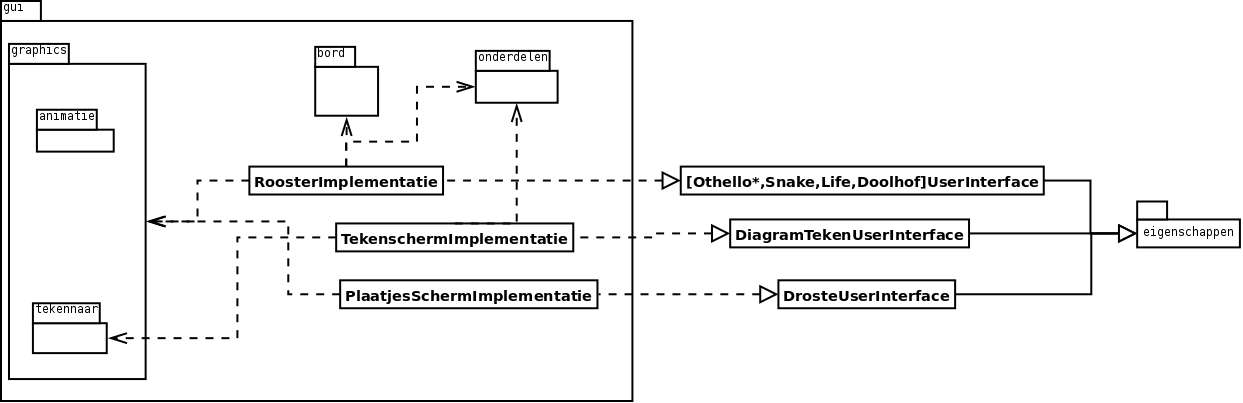
\includegraphics[width=1.3\linewidth]{Diagram1.png}
 % Diagram1.png: 1243x403 pixel, 51dpi, 62.15x20.15 cm, bb=0 0 1762 571
\end{center}

\end{figure}

\section{Top-Level}

Hierboven zie je hoe het ui package er op een high-level uit ziet. De diverse UserInterface interfaces extenden de diverse eigenschappen (multiple inheritance kan bij interfaces). Die eigenschappen bestaan alleen maar om er voor te zorgen dat bij Userinterfaces die dezelfde methodes hebben niet de hele tijd de methodes gekopieerd worden en we zo een onoverzichtelijke java doc krijgen. \\

\begin{itemize}

\item Alle Userinterfaces die een rooster op het scherm krijgen (Life, Othello*, Snake, Doolhof) worden allemaal geimplementeerd door de class RoosterImplementatie.
\item De DrosteUserinterface wordt geimplemeneerd door PlaatjesSchermImplementatie.
\item De DiagramUserInterface wordt geimplementeerd door TekenSchermImplementatie.
\item De StaafDiagramUserInterface wordt geimplemeerd door StaafDiagram in het package ui.gui.staafdiagram, en deelt geen code met de rest van de UserInterfaces.
\end{itemize}

\begin{itemize}
 \item De RoosterImplementatie gebruikt beide packages (animatie en tekennaar) uit de gui.
\item Net als de PlaatjesSchermInterface
\item De TekenSchermImplementatie heeft geen animaties en gebruikt dus alleen tekennaar.
\end{itemize}

In het package onderdelen zitten classes voor het verwerken van events en een statusbar, deze worden gebruikt door RoosterImplementatie en TekenschermImplementatie maar niet door PlaatjesSchermImplementatie aangezien die geen events of statusbar heeft.\\

In Bord zitten classes voor de RoosterImplemenatie om te gaan met de vakjes.


\section{Graphics}

In het package ui.graphics zitten classes die door alle userinterfaces gebruikt worden om elementen op het scherm te tekenen.

\subsection{Tekennaar}

In het package ui.graphics.tekennaar zitten diverse classes die als functor gebruikt kunnen worden om te tekenen. Dat wil zeggen dat de classes eigenlijk een soort wrapper om een methode om te tekenen zijn, het voordeel hiervan is dat we gemakkelijk methodes om te tekenen kunnen doorgeven en gebruiken als argumenten naar functies e.d. Alle tekennaars implementeeren de interface tekennaar:

\begin{verbatim}
 public interface Tekennaar {
     void teken(Graphics2D g);
     
     Dimension geefAfmetingen();
     
     boolean bevat(Point point);
     
}
\end{verbatim}


Dus ze hebben een methode teken die gegeven een graphics2D object (dat geeft swing je in een paint methode) wat op het scherm kunnen tekenen. Bijvoorbeeld de functor om een groene half doorzichte cirkel op 0,0 en een roode lijn van 400,200 naar 700,500 te tekenen ziet er zo uit:

\begin{verbatim}
           Tekennaar bla = new CombinatieTekenaar(
                    new AlphaTekennaar(
                              new KleurTekennaar(Color.GREEN, 
                                        new CirkelTekenaar(30,30,true))
                              ,0.5f),
                    new TranslatieTekennaar(
                              new KleurTekennaar(Color.RED,
                                        new LijnTekennaar(300, 300)), 
                              400,200)
                    );
\end{verbatim}

Deze tekennaar (bla) kunnen we dan doorgeven om aan te geven wat er getekend moet worden. Bijvoorbeeld bij TekenSchermImplementatie houd die class enkel 1 (Combinatie) tekennaar bij waarin staat wat de gebruiker allemaal op het scherm wil tekenen en als dat paint door swing wordt aangeroepen roepen we de teken( ..) methode van die tekennaar aan.

\subsection{Animatie}

Voor de fade en clip-in effecten op bij het rooster en bij droste worden animatie ojbecten gebruikt uit ui.gui.graphics.animatie  Het essentiele punt hiervan is de volgende interface:

\begin{verbatim}
 public interface TransitieDeelTekenaarMaker{
     Tekennaar geefTekennaarOpDeel(Tekennaar tekennaar,float deel);
}
\end{verbatim}

De bedoeling is dat zo'n object de tekennaar geeft op een bepaalt gedeelte van de animatie. Bijvoorbeeld een alphatransitie op een willlekeurige tekenaar (zoals bij othello):

\begin{verbatim}
      public static class AlphaTransitie implements TransitieDeelTekenaarMaker{
          public Tekennaar geefTekennaarOpDeel(Tekennaar tekennaar, float deel) {
               return new AlphaTekennaar(tekennaar,deel);
          }
     }
\end{verbatim}

Om een animatie te maken hoeven we dan alleen maar de oude tekennaar en de nieuwe tekennaar (dus bijv een tekennaar voor een wit othello steentje en een lege tekennaar) zodat het steentje verdwijnt en een inTransitie deelTekennaarMaker (de deel tekennaar voor de animatie om te verschijnen van de nieuwe tekennaar) en de uit transitie(vice versa) tekennaarmaker plus de tijd dat het moet duren aan een animatie object te geven. Daarop kunnen we net als een tekenaar de teken(..) aanroepen, het animatie object houd de tijd bij en teken de tekennaar met de juiste aanpassingen voor de animatie (dus bijv. het deel van animatie = 0.6 van de totale tijd dus  de inTekenennaar tekenen we 0.6 doorzichtig en de outtekenaar 0.4 doorzichtig).\\

Zo'n animatie object kunnen we dan ook weer doorgeven etc. Hieronder een voorbeeldje uit de plaats(..) van PlaatjesSchermImplementatie. De nieuwe tekenaar is dus het plaatje en de oude tekennaar is niks. Voor zowel in doen we een fade( alpha) transitie en voor uit doen we niks. De tijd die de animatie mag duren is de tijd die de gebruiker met wacht(..) heeft ingevoerd.

\begin{verbatim}
 
          public void plaats(BufferedImage plaatje, int x, int y,
                    int breedte , int hoogte){
               double scaleX = (double) breedte / (double) plaatje.getWidth();
               double scaleY = (double) hoogte / (double) plaatje.getHeight();
               Animatie animatie = 
                    new Animatie(new TransitieVerzameling.AlphaTransitie(), 
                         new TransitieVerzameling.GeenTransitie(), 
                         new TranslatieTekennaar(
                                   new ScaleTekennaar(scaleX,scaleY,
                                             new PlaatjeTekennaar(plaatje)),x,y), 
                         new NiksTekennaar(),
                         schermVerversDuratie , 
                         schermVerversDuratie);
               synchronized (animaties) {
                    animaties.add(animatie);
               }
               repaint();
          }

\end{verbatim}


\section{Instellingen voor RoosterImplementatie}

Omdat de roosterSchermImplementatie een aantal verschillen userinterfaces implementeerd wordt er om de roosterscherm het goede gedrag te laten hebben gebruik gemaakt van instelling objectjen.:

\subsection{VakjeGraphics}

Om in te stellen wat er in een vakje van het rooster (bijv ui.PAD, ui.LEEG , ui.SNAKE etc) te zien zien hebben we de VakjeGraphics class

\begin{verbatim}
 public class VakjeGraphics {
     public Tekennaar tekenaar;
     public TransitieDeelTekenaarMaker animatieInKeuze;
     public TransitieDeelTekenaarMaker animatieOutKeuze;
     public double animatieInFactor; 
     // hoeveel tijd van de wacht(..) moet er gebruikt worden?
     // bijv 0.5 als de wacht 200 ms is dan duurt de animatie 100ms
     public double animatieOutFactor;

}
\end{verbatim}

Hij heeft dus een tekennaar met wat er te zien is (bijv. wite othello steen) en animaties voor als de vakjeGraphics van het vakje veranderd wordt (als er veranderd wordt worden de animaties van de nieuwe vakjegraphics gebruikt) Dit is geimplemeert in ui.gui.bord.Hokje. 

\subsection{Map}

Om de integer constanten (bijv ui.PAD, ui.LEEG , ui.SNAKE etc)  aan de vakjegraphics te binden gebruiken we een Map object dat van Integer naar een VakjeGraphics gaat. Bijvoorbeeld bij de OthelloReplay userinterface hebben we een map object dat gegeven ui.WIT de vakjeGraphics voor een witte steen teruggeeft. Dit map object geven we dan aan roosterSchermImplementatie en dan laat hij bij ui.plaatst(44,3, ui.WIT) daar een witte othello steen zien. \\

Voor de omcirkelingen is net zo'n Map, maar dan van Boolean naar VakjeGraphics\\

De twee vakjeGraphics worden overelkaar heen getekend (dus eerst bijv. de steen, dan de omcirkeling)

\subsection{GUIInstellingen}

Al deze instellingen komen samen in de GUIInstellingen class waar alle instellingen voor RoosterSchermImplemenatie in staan. Dus een Tekenaar voor de achtergrond een map voor wat er in de vakje kan komen etc:

\begin{verbatim}
 

public class GUIInstellingen {
     
     static final double STANDAARD_ANIMATIE_BEELDEN_PER_SECONDE = 30.0;
     
     public double animatieBeeldenPerSeconde;
     /* hangt de duratie van de animatie af van beelden per seconde die de
      * gebruiker zet of de waarde van wacht(..) of niet?
      */
     public boolean animatieSchermVerversen;
     // alleen als animatieSchermVerversen uit staat:
     public int animatieDuratie;
     
     public OmcirkelMap omcirkelMap;
     public KleurMap map;
     // Tekennaar voor respecievelijk de achtergrond en de voorgrond
     public Tekennaar bordUnderlay, bordOverlay;
     public int breedte,hoogte;
     // geven we events?
     public boolean interactief;
     
     public boolean tekenOmcirkelBovenNormaal;
     /* geven we bij een mouse over etc. event de coordinaat in a 3 of in 0 2? */
     public boolean lettersVoorHorizontaleCoordinaten;
     public boolean pasKnopje;
     
     public String titel;
     
     public int horizonaleHokjeSpacing, verticaleHokjeSpacing;
     public int horizontaleLinksInspring, horizontaleRechtsInspring,
          verticaleBovenInspring, verticaleOnderInspring;
     public Dimension hokjeAfmetingen;
\end{verbatim}

De instellingen voor de UserInterfaces op een RoosterScherm staan in ui.gui.instellingen

\section{Events}

Het belangrijkste onderdeel van het evensysteem is ui.gui.onderdelen.GUIInstellingen. Deze class houd een queue bij van alle events bij. Elk object dat events kan genereren (bijv. Hokje (mouseover, klik), UIKeyListner , StatusBar (pas knop), AlarmSysteem) krijgt een referentie naar dit object (er is er dus maar 1 van). Via dit object voegen zij events toe aan de queue en vervolgens vraagt de RoosterImplementatie of TekenSchermImplemenatie aan dit object om events. Als er geen event is blokken we. 

\end{document}          
